\subsection{Convolutional Neural Networks}
  Convolutional Neural networks(CNN) have been prominent in the field of Computer vision in recent years.
  CNNs have been used in field of computer vision in order to classify images with high accuracy and speed \cite{razavian2014}.
  CNNs come at the cost of requiring long times to train, in most cases using GPUs \cite{krizhevsky2012}.
  This makes standard use of CNNs impractical for tracking unknown objects, training a CNN online results in impairment of the system's speed \cite{bertinetto2016}.

  \subsubsection{Crowd Segmentation with CNNs}
  A crucial part of a tracking is the ability to distinguish background from objects of interest.
  \citeauthor{kang2014} \cite{kang2014} propose fast fully convolutional neural networks(FCNN) to segment crowds.
  The FCNN allows for a whole image to be searched in one pass of forward propagration.
  This allows faster and more accurate segmentation in comparison to sliding window techniques.

  The FCNN has no fully connected layers in the CNN, instead it uses a $1 \times 1$ convolution kernel layer to predict labels.
  This removes the translation dependence of CNNs that is due to the fully connected layers.
  The translation invariance of the network allow the single pass of the image.

  This technique uses appearance to segment the crowd--this reduces the false positives which occur when motion cues are used to segment crowds.
  Another advantage of scanning the whole input image once is the availability of more contextual appearance information which can be used in segmentation \cite{eigenFacesRecog, farabet2012}.
  Once an image of a crowd is segmented, more specific analyisis can be done, for example identification of people in the crowd.


  \subsubsection{Multi-domain CNN}
  \citeauthor{CNNTracking} \cite{CNNTracking} use a CNN as the basis of a tracker(MDNet) that they implement.
  The CNN is trained on a large, labelled dataset of videos to obtain generic target representations.
  Training is done on one separate domain, cars for example, at a time. 
  All the domains are worked through in an iterative process.
  This provides a CNN that can distinguish between a target, from any of the trained domains, and background.

  \begin{figure}[!ht]
    \centering
    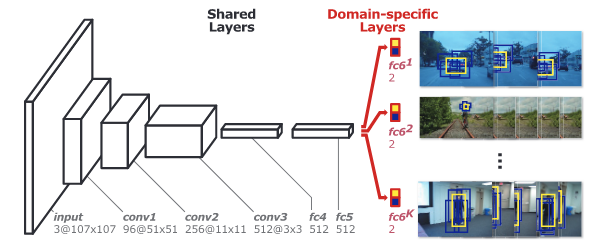
\includegraphics[scale=0.5]{MDNet.png}
    \caption{The architecture of the Multi-Domain Network, from \protect\cite{CNNTracking}}
    \label{fig:mdnet}
  \end{figure}
  The output of this CNN is branches into input for domain-specific layers, see Figure~\ref{fig:mdnet}.
  These output layers are binary classifiers that use the CNN's generic representation to track a target in a specific domain.
  These layers are trained online using the video stream as input, in order to improve the tracker's accuracy as the video progresses.

  This design allowed \citeauthor{CNNTracking} to get very high accuracy in VOT challenges.
  The high accuracy comes at the cost of real time execution--the binary classifers of the network require a lot of time to train online.
  MDNet was only able to process one frame per second in the VOT challenges \cite{bertinetto2016}, this makes in unsuitable for real-time tracking.
  

  \subsubsection{Convolutional Siamese Neural Networks}
  \citeauthor{bertinetto2016} \cite{bertinetto2016} offer a solution to the problem of tracking an unknown object with Convolutional Neural networks.
  The solution given by \citeauthor{bertinetto2016} is to train, offline, a CNN that solves the more general similarity problem.
  A similartiy function $f(z,x)$ is learned, the funtion compares images $x$ and $z$ and returns values that estimate how similar the images are.
  This function can be considered as a composition of two other functions $f(z, x) = g(\phi(z), \phi(x))$.
  In this composition, $\phi$ is an embedding that does the convolution and $g$ is a metric.
  A siamese neural network, two identical neural networks conjoined at the output node \cite{bromley1993}, is used to learn the similarity relation.

  A \textit{fully-convolutional}, translation invariant, siamese network is suggested by \citeauthor{bertinetto2016}.
  The input to the network is an image centered on the target's previous location.
  The network outputs a score map represented as a grid of numbers, Figure~\ref{fig:convSiamese}.

  \begin{figure}[!ht]
    \centering
    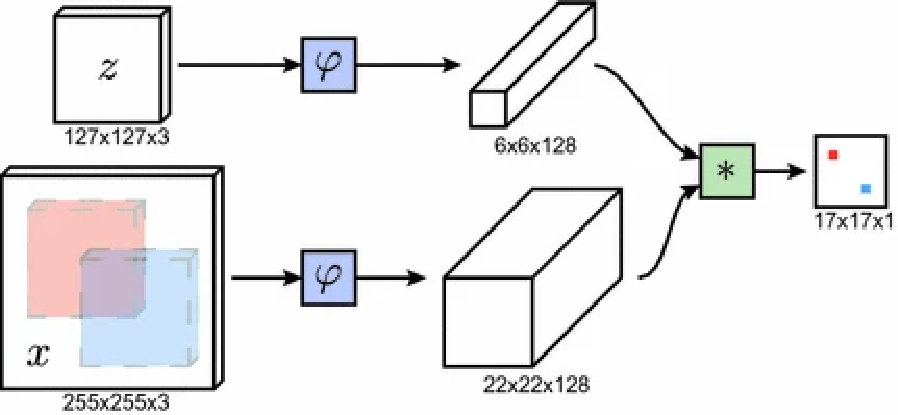
\includegraphics[scale = 0.6]{convSiamese.pdf}
    \caption{The architecture of the Fully Convolutional Siamese Neural Network, from \protect\cite{bertinetto2016}}
    \label{fig:convSiamese}
  \end{figure}

  This architecture can be seen as an advanced template tracker.
  The CNN is equivalent to the preprocessing needed to create a tracking template.
  The metric $g$ compares the template and a search window--the sum of squares metric is often used in template trackers.

